\documentclass[11pt, oneside]{article}
\usepackage{titling, hyperref, geometry, amsmath, amssymb, algorithm, graphicx, textcomp, subcaption}
\usepackage[noend]{algpseudocode}
\usepackage[cache=false]{minted}
\geometry{a4paper}

\hypersetup{
    colorlinks=true,
    urlcolor=cyan
}

\newcommand{\emphasis}[1]{\textcolor{blue}{\textbf{\textit{#1}}}}

\title{String Matching}
\author{Stephen Huan \\ Edited by: Udbhav Muthakana}

\begin{document}
\maketitle

\section{Definition}
Let \( T \) be a string of length \( m \) and \( P \) a string of length \( n \).
We assume both strings only contain characters from a finite alphabet \( \Sigma \),
e.g. \( \Sigma = \{ 0, 1 \} \) for binary and \( \Sigma = \{ A, G, C, T \} \) for DNA.
The \emphasis{string-matching problem} is then defined as finding every index \( i \)
such that \( T[i \dots i + n] = P \), i.e. the substring of \( T \) starting at that index is
equal to the pattern string \( P \).

We can further generalize the problem to include multiple pattern strings, \( P_1, P_2, \dots P_k \). We define \( n \) to be \( \Sigma^{k}_{i = 1} |P_i| \) and define the output to be the matches for each pattern string, with a total number of \( z \). Note that \( z \) in the worst case can be
\( O(n^2) \): take the example of \( T = \text{aaa\dots a} \) and \( P_1 = \text{a}, P_2 = \text{aa}, P_3 = \text{aaa}, \dots \)

\begin{table}[h!]
\centering
\begin{tabular}{ ccc }
 Algorithm & Preprocessing time & Matching time \\
 \hline
 Naïve & \( 0 \) & \( O(nm) \) \\
 Rabin-Karp & \( \Theta(n) \) & \( O(nm) \) \\
 Finite automaton (naïve) & \( \Theta(n|\Sigma|) \) & \( \Theta(m) \) \\
 Knuth-Morris-Pratt (KMP) & \( \Theta(n) \) & \( \Theta(m) \) \\
 Aho-Corasick & \( \Theta(n) \) & \( \Theta(m + z) \) \\
 Suffix Tree & \( \Theta(m) \) & \( \Theta(n + z) \) \\
 Suffix Array & \( \Theta(m) \) & \( O(n + \log m + z) \) \\
 \hline
\end{tabular}
\caption{String-matching algorithms}
\end{table}

A common notation for running time of algorithms is \( \langle f, g \rangle \)
where \( f \) is the preprocessing time and \( g \) is the execution time. Thus, Aho-Corasick has a running time of \( \langle O(n), O(m + z) \rangle \).

\newpage

\section{Algorithms}
\subsection{Naïve}

\begin{algorithm}
  \begin{algorithmic}[h!]
    \Procedure{Naive-String-Matcher}{$T$, $P$}
      \For{each position in T}
          \For{each pattern string $P_i$}
            \State check for a match
          \EndFor
      \EndFor
    \EndProcedure
  \end{algorithmic}
\end{algorithm}

For each character in \( T \), in the worst case we go over each \( n \)
characters making the running time \( O(nm) \). Intuitively, this is slow
becuase information about \( T \) doesn't carry over to each string.
For example, if the first character of \( T \) is ``a'', our ideal algorithm should
elimate all patterns that don't start with ``a'' and propagate the constraint
forward for all patterns that do. How do we actually implement this ``parallel'' searching?

\begin{figure}[h!]
\centering
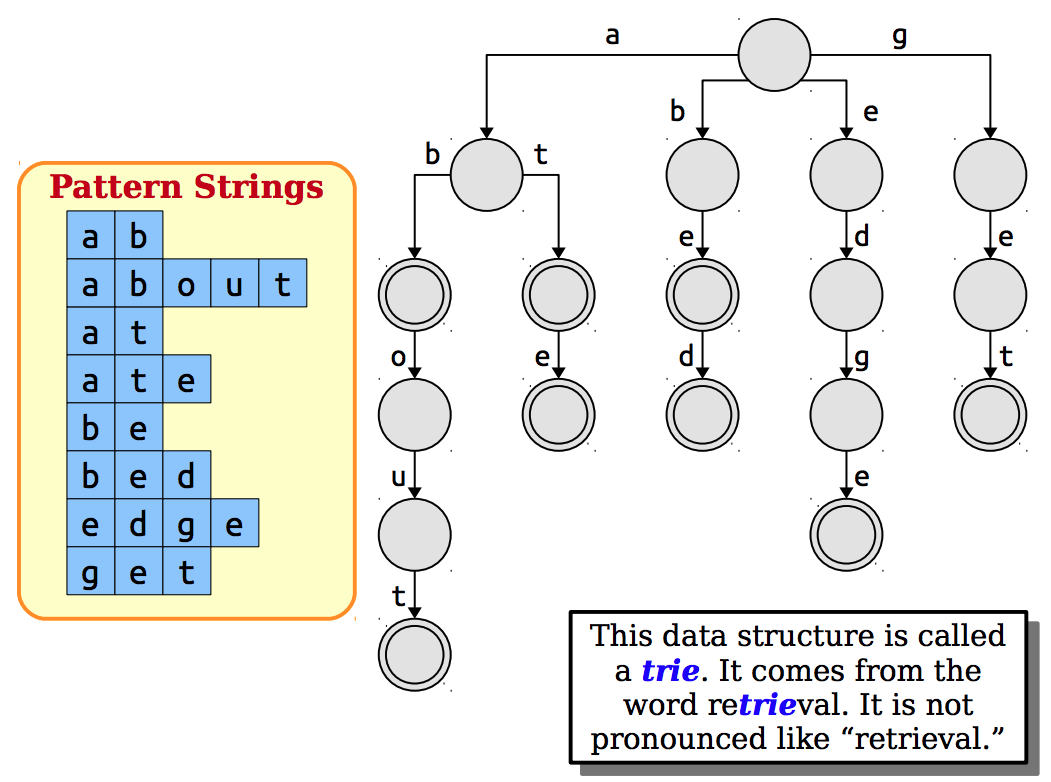
\includegraphics[scale=0.25]{trie}
\caption{The trie data structure}
\end{figure}

There are a variety of simple ways to represent a \emphasis{trie}.
One way to represent child pointers is a character array of length \( |\Sigma| \),
but that would make construction time \( O(n |\Sigma|) \), as each character would have its own array.
Instead, we can represent children by a character map, making construction \( \Theta(n) \).

To search with the trie, for each position in \( T \) we propagate a pointer from the root down the trie as far as possible (until it is no longer in the trie).
Each node maintains whether it is the end of a pattern word, and on reaching an end node we report a match.
This algorithm runs in \( O(m L_\text{max}) \), where \( L_\text{max} \) is the length of the longest pattern string.

\subsection{Suffix Links}

The previous trie algorithm was slow because it restarted at the root for each character.
Instead, we can keep track of nodes to go back to in the event of ``failure'' (character mismatch).

A \textbf{\textit{suffix link}}, indicated by a red edge, is defined as a edge between a trie node that represents a string \( \alpha \)
and another trie node that represents \( \omega \), such that \( \omega \)
is the longest proper suffix of \( \alpha \) in the trie. A ``proper'' suffix
is a suffix that isn't the original string. A suffix link must be proper because a trie can't have
distinct nodes which represent the same string - they'd occupy the same node.

Intuitively, on a character mismatch, we can follow suffix links to preserve as much context as possible.
The root corresponds to the empty string \( \epsilon \) and is the only node that doesn't have a suffix link.

\begin{figure}[h!]
\centering
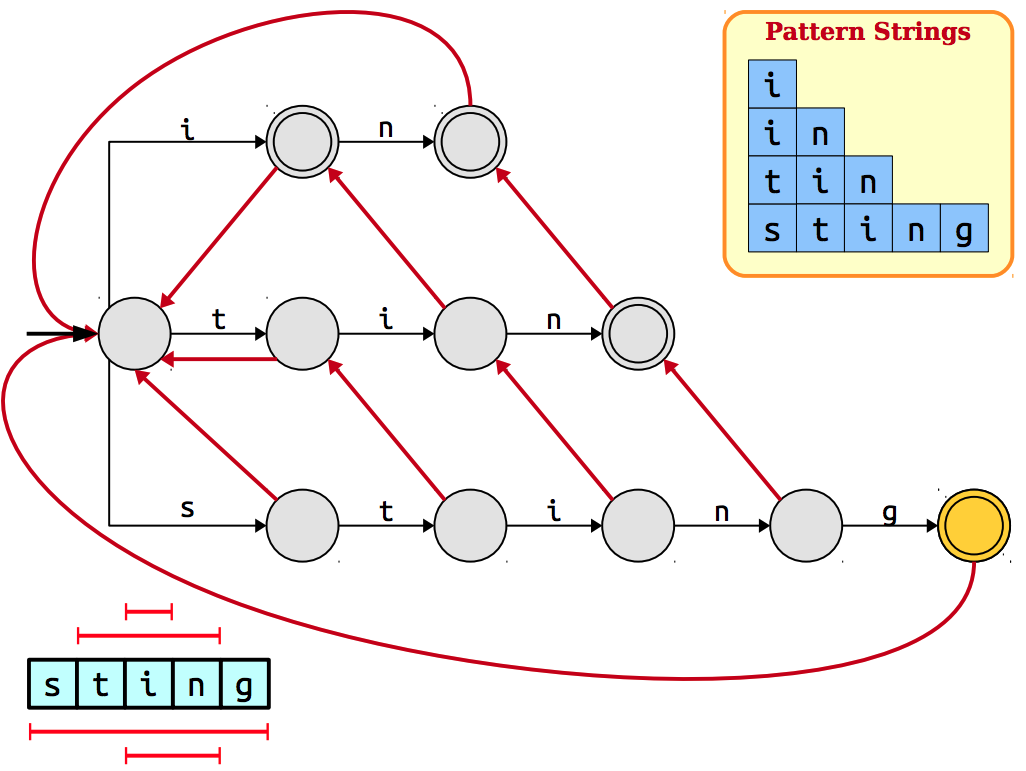
\includegraphics[scale=0.25]{suffix}
\caption{Trie with suffix links shown}
\end{figure}

To search with suffix links, start at the root and propagate a pointer
forward for each position in \( T \). When there is mismatch, follow suffix links back through the trie until you reach the root
or you no longer mismatch.

To analyze the running time of this algorithm, note that the pointer can go
at most \( m \) forward into the trie, as it moves exactly one character forward on a match.
In the worst case, each suffix link moves the pointer one back, making the
number of ``fallback'' steps at most \( m \), as the suffix links can't move the pointer past the root.
Thus, the algorithm runs in \( \Theta(m) \).

\newpage

\subsection{Output Links}

Since suffix links no longer start searching at each position,
certain patterns can be skipped (those that are suffixes of other patterns).
To account for this, create \\ \emphasis{output links} associated with each node by using
the existing suffix links.
When a node is visited, output all the nodes in the linked list formed by the output links.

\begin{figure}[h!]
\centering
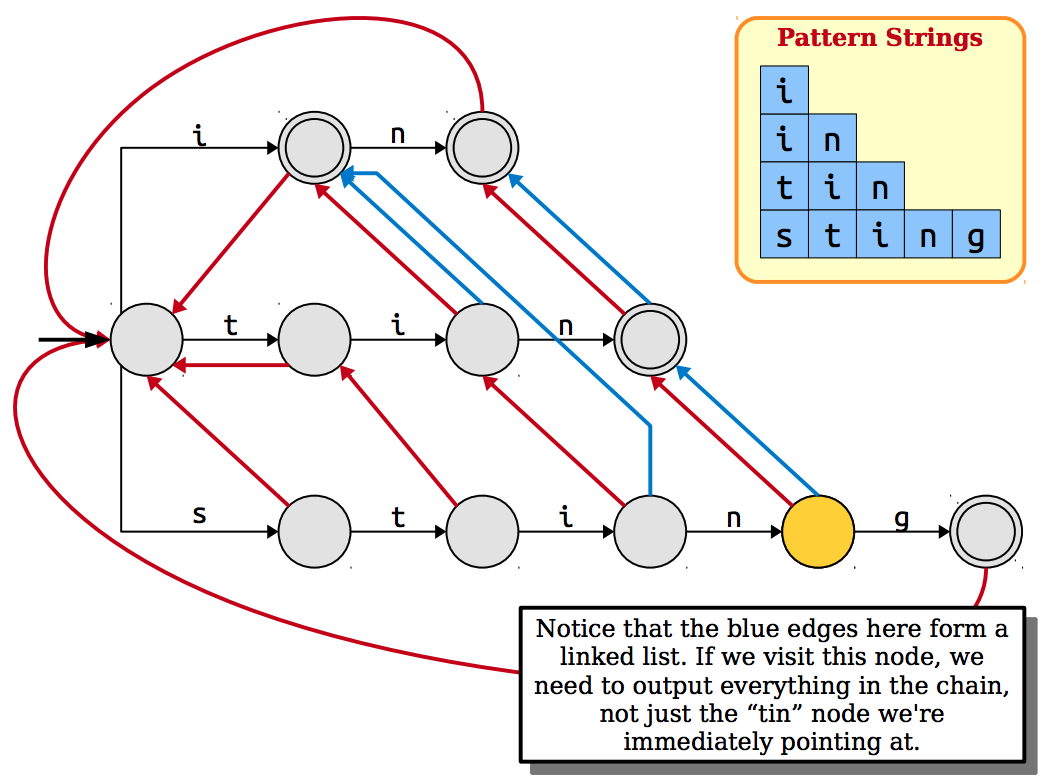
\includegraphics[scale=0.25]{output}
\caption{Trie with output links shown}
\end{figure}

\subsection{The Final Matching Algorithm}

\begin{itemize}
    \item Start at the root
    \item For each character \emphasis{c} in the string:.
      \begin{itemize}
        \item While there is no edge labeled \emphasis{c} and you're not at the root:
          \begin{itemize}
            \item Follow a suffix link
          \end{itemize}
        \item If there's an edge \emphasis{c}, follow it.
        \item If the current node corresponds to a pattern, output it.
        \item Output all words in the chain of output links originating at this node.
      \end{itemize}
\end{itemize}

\newpage

\subsection{Constructing links}

In order to construct suffix links, we'll use an approach that is essentially dynamic programming.
Suppose we have a node that ends with a character \( a \) and therefore represents the word \( wa \).
In order to compute its suffix link, we can use the suffix link of \( w \).
We follow \( w \)'s suffix link to some node \( x \). If \( xa \) exists, then \( wa \) has a suffix link
to \( xa \). Otherwise, follow \( x \)'s suffix link. If we reach the root,
then \( wa \)'s suffix link points to the root.

Suffix links must point from longer strings to shorter strings, because a proper suffix of a string
must be shorter than the string. Therefore, maintain the base case of the root having no suffix links
and the root's children's suffix links pointing to the root. Run a breadth-first search on the trie,
and compute the suffix links with the above logic.

The output link of a node \( w \) points to the longest proper suffix of \( w \) that is a pattern,
or null otherwise. Since it points to the \textit{longest} suffix, we can reach all patterns
by a linked list of output links. To construct output links, initialize all of them to null.
While BFS'ing to construct suffix links, use the following logic for a node \( u \):
Let \( v \) be the suffix link of \( u \). If \( v \) is a pattern, \( u \)'s output link
points to \( v \). Otherwise, \( u \)'s output link points to the output link of \( v \).

The analysis of the efficiency of this algorithm is similar to the analysis of the pattern matching algorithm.
The bound on the number of steps backwards following suffix links is the number of steps forward, which is exactly \( n \).
Therefore, the running time of the algorithm to generate suffix and output links is \( O(n) \).

The resulting graph is known as an \emphasis{Aho-Corasick automaton} beacuse it is a specific way to construct
a finite state automaton.

A sample implementation of this algorithm along with KMP is given \href{https://gist.github.com/stephen-huan/aa609965c86d750736398c28b025f9be#matching}{here}.

\section{Comparision to Other Algorithms}

Obviously, Aho-Corasick dominates the naïve algorithm. Knuth-Morris-Pratt is a specific instance of
Aho-Corasick for one pattern word (the trie becomes a linked list and can be represented by an array).
Some may find Rabin-Karp easier to program, but it is mathematically motivated, uses hashing,
and in the worst case can be very slow.

Use Aho-Corasick when you have set pattern strings and a changing target string,
and use suffix trees/arrays when you have a set string but changing patterns.

\newpage

\section{Sample Problems}

\begin{enumerate}

  \item \href{https://onlinejudge.org/index.php?option=onlinejudge&page=show_problem&problem=1620}{UVa 10679: I Love Strings!!}:
  Given a target string of length \( \leq 10^5 \) and at most 1,000 pattern strings of length at most 1,000, say for each pattern
  whether or not it's a substring of the target string.

  The obvious solution is to use Aho-Corasick on the patterns and then run it over the target string.
  There are only three complications:
  \begin{enumerate}
    \item They consider the empty string to not be in the target string.
    \item There can be duplicated words. To account for this, maintain a list of words for each trie node.
    When matching a word, add the match to every word in the node's list.
    \item In the worst case - the target string is aaa...aaa and \( 10^5 \) long and each of the \( 10^3 \) patterns is ``a'' -
    there are \( 10^3 \cdot 10^5 \) matches which will not run in time. However, note that we only need to report
    whether a pattern is a substring e.g. if it appears 0 or \( \geq 1 \) times. Maintain a set of seen nodes and skip traversing their output links.
    Also maintain a set of seen indexes and skip adding matches to the rest of the items in the same list.
    Both sets guarantee that each pattern is only matched once, making our total complexity  \( O(m) \) instead
    of \( O(m + z) \) and allowing the algorithm to run in time.
  \end{enumerate}

  Note that there is a more optimal way to keep track of duplicate words
  (think of the extreme example given previously - if you wanted the number of matches,
  then you could match just one of the words and copy the answer for the duplicates).
  Still maintain a list of words for each trie node, but only update the first pattern's count.
  At the end, run a DFS, and for each other pattern in the list, set their matches to the first pattern in the same list.

  \item \href{http://www.usaco.org/index.php?page=viewproblem2&cpid=533}{USACO Censoring}:
  Given a string \( s \) with length at most \( 10^5 \) and a list of pattern words such that no pattern
  is a substring of another pattern and the total length is at most \( 10^5 \), create a new word
  by repeatedly finding the first instance of a pattern in \( s \) and removing it.

  Solution: Construct an Aho-Corasick automaton from the patterns and scan \( s \) from left to right, adding
  characters of \( s \) to a stack. On a match, remove the length of the matched word from the stack.
  Then, restore the state of the automaton by maintaining an table mapping an index to a trie node.
  Use this table to go back to the last character after removing the matched word.

  Recall that in our original formulation for the Aho-Corasick string matching algorithm,
  we allowed backtracking because it would be bounded by the amount it moved forward.
  Since we jump to the last state after removing a word, we no longer have a linear bound
  on the amount of backtracking. Therefore, you will need to also maintain another transition table,
  caching the transition from a trie node given a new character.

  \item (CLRS)/\href{https://www.spoj.com/problems/EC_WORLD}{SPOJ Rotations}: Give a linear time algorithm for determining whether one string is a cyclic rotation of another.

  Solution: First of all, both strings must have an equal length called \( m \).
  Consider generating all \( m \) possible cyclic rotations of one of the strings: the problem
  then becomes detecting whether any of them are equal to the other string. Instead of
  actually generating these strings, we can represent a cyclic rotation by its starting index.
  The cyclic string is then the string formed by starting at that index, traversing to the end,
  then wrapping back around to that index. However, simulating this out would be slow.
  The key observation is that the last cycle would be at the very end of the string
  and has a length of \( m \). Therefore, all cycles must finish within the original string doubled:
  e.g. if the string is ``car'', all of its cycles (``car'', ``arc'', and ``rca'') are substrings of ``carcar''.

  The solution is then to pick a string, add it to itself, and see if the other string is a substring of the doubled string
  and has equal length. Pick whatever linear matching algorithm you want - the simplest is probably KMP.

  \item \href{https://codeforces.com/problemset/problem/126/B}{Codeforces 126B}: Asterix, Obelix, and their new friends Prefix and Suffix
  want to find a special substring \( t \) of larger string \( s \) (\(1 \leq |s| \leq 10^6 \)).
  This must be the longest substring that appears as a prefix, as a suffix, and as neither.
  Print one such substring or say that none exists.

  Solution: I have an LCP-array theoretic solution that runs in \( O(m) \), but sadly the suffix array construction is too slow. I'm told this problem can be solved with either the prefix function of KMP or the Z-function. Figure it out!

  \item \href{https://contest.usaco.org/DEC05.htm}{USACO 2005 Cow Patterns} (\href{http://poj.org/problem?id=3167}{POJ link}): Farmer John has lined up his \( N \) (\( 1 \leq N \leq 10^5 \)) cows,
  looking for a particular substring of \( K \) (\( 1 \leq K \leq 25,000 \)) cows.
  Each cow has some number of spots \( S \) (\( 1 \leq S \leq 25 \)), but he does
  not remember the exact numbers of the \( K \) cows, only their relative ranking. For example, he might
  remember the sequence 1 4 4 3 2 1. This means cows 1 and 6 had the same numbers, as did 2 and 3,
  and 2 had more spots than 4, who had more spots than 5.
  Find the number of substrings of the \( N \) cows consistent with the \( K \)-long ranking.

  \href{https://contest.usaco.org/DEC05anal/cpattern.htm}{Solution}: Use a modified KMP.

\end{enumerate}

\newpage

\section{Past Lectures}

\begin{enumerate}
  \item \href{https://activities.tjhsst.edu/sct/lectures/1617/2017-06-02_Aho_Corasick.pdf}{``Aho-Corasick'' (Neil Thistlethwaite, 2017)}
  \item \href{https://activities.tjhsst.edu/sct/lectures/1516/SCT_Aho_Corasick.pdf}{``Aho-Corasick'' (Lawrence Wang, 2016)}
  \item \href{https://activities.tjhsst.edu/sct/lectures/1718/2017-10-27_String_Searching.pdf}{``String searching'' [KMP and Rabin-Karp] \\ (Larry Wang and Charles Zhao; presented by Mihir Patel, 2017)}
  \item \href{https://activities.tjhsst.edu/sct/lectures/1415/stringmatching_10_3_14.pdf}{``String Matching Algorithms'' [KMP and Rabin-Karp] \\ (Hariank Muthakana and Corwin de Boor, 2014)}
  \item \href{https://activities.tjhsst.edu/sct/lectures/1314/string_matching_11_01_13.pdf}{``String Matching'' [KMP and Rabin-Karp] (Sreenath Are, 2013)}
  \item \href{https://activities.tjhsst.edu/sct/lectures/1112/string.pdf}{``String Algorithms'' [KMP, Z algorithm] (Nick Haliday, 2012)}
  \item \href{https://activities.tjhsst.edu/sct/lectures/1112/strings111811.pdf}{``Cool String Tricks'' [Rabin-Karp and Tries] (Alex Chen, 2011)}
  \item \href{https://activities.tjhsst.edu/sct/lectures/1617/2016-11-11_String_Searching.pdf}{(Broken) String searching (Larry Wang and Charles Zhao, 2016)}
\end{enumerate}

\section{Works Cited}

\begin{enumerate}
  \item \href{http://web.stanford.edu/class/archive/cs/cs166/cs166.1166/lectures/02/Small02.pdf}{Stanford lecture on Aho-Corasick}
  \item \href{https://web.stanford.edu/class/cs97si/10-string-algorithms.pdf}{``String Algorithms''} by Jaehyun Park for CS 97SI at Stanford
  \item \href{https://mitpress.mit.edu/books/introduction-algorithms-third-edition}{\textit{Introduction to Algorithms}} (also known as CLRS)
\end{enumerate}

\end{document}
